%!TEX TS-program = xelatex
%!TEX encoding = UTF-8

% Template for the class file AJbook, originally designed for Chinese book ``代数学方法''.
% Copyright 2018  李文威 (Wen-Wei Li).
% Permission is granted to copy, distribute and/or modify this
% document under the terms of the Creative Commons
% Attribution 4.0 International (CC BY 4.0)
% http://creativecommons.org/licenses/by/4.0/

% 使用自定义的文档类 AJbook.cls. 自动载入 xeCJK. 需要额外档案如下:
% font-setup-open.tex, coverpage.tex, titles-setup.tex, mycommand.sty, myarrows.sty
% 文档类选项 (key/val 格式):
% draftmark = true (未定稿, 底部显示日期) 或 false (成品), 默认 false,
% colors = true (链接带颜色无框) 或 false (黑色无框), 默认 true,
% traditional = true (繁体中文) 或 false (简体中文), 默认 false,
% coverpage = 封面档档名, 默认为空 (此时不制作封面), 一般是 .tex 档, 若为 *.pdf 的形式则直接引入 PDF 页面.
% fontsetup = 字体设置档档名,
% titlesetup = 章节格式设置档名.

% 注意: 如果文中未使用 \cite 和 \index 命令, 则可能报错.

% 需动用 imakeidx + xindy (两份索引), biblatex + biber (书目). 
% 索引用土法进行中文排序: 如 \index{zhongwen@中文} 等.
\documentclass[
	draftmark = false,   % 草稿模式下, 每页底部将打印相关版本信息.
%	traditional = true,
%	colors = false,
%	coverpage = coverpage.tex,
%	coverpage = coverpage.pdf,
%   geometry = b5,    % 版面设置, 目前仅容许 a4, b5, 默认 b5, 其它字串则不作自动设置.
	fontsetup = font-setup-open.tex,
	titlesetup = titles-setup.tex
]{AJbook}

% 可以修改章节编号的深度
% \setcounter{secnumdepth}{3}

% 必要时仅引入部分档案
% \includeonly{}

% 生成索引: 选用 xindy + imakeidx
\usepackage[xindy, splitindex]{imakeidx}
\makeindex[
	columns=2,
	program=truexindy,
	intoc=true,
	options=-M texindy -I xelatex -C utf8,
	title={名词索引}]	% 名词索引

\usepackage[unicode, bookmarksnumbered]{hyperref}	% 启动超链接和 PDF 文档信息所需
% 设置 PDF 文件信息
\hypersetup{
	pdfauthor = {Lichuang},
	pdftitle = {Latex 数学符号、排版cheat sheet},
	CJKbookmarks = true}

% 增加表格高度
\renewcommand*\arraystretch{1.5}

% 自订公式的编号 (非必要)
\numberwithin{equation}{section}
\renewcommand{\theequation}{\thesection--\arabic{equation}}

% 图片相关的宏包
\usepackage{graphicx} %插入图片的宏包
\usepackage{float} %设置图片浮动位置的宏包
\usepackage{subfigure} %插入多图时用子图显示的宏包

% 自订 figure 的编号 (非必要)
%\numberwithin{figure}{section}
%\renewcommand{\thefigure}{\thechapter--\arabic{figure}}

% 自订 table 的编号 (非必要)
%\numberwithin{table}{section}
%\renewcommand{\thetable}{\thechapter--\arabic{table}}

\begin{document}
	\frontmatter	% 制作封面和目录.
	% 注意: 为了简化, 本模板不含封面. 请通过文档类的参数进行设置.
	
	\mainmatter		% 正文开始:逐章引入 TeX 代码

	\chapter{数理逻辑符号}
	\newcommand\tauteq{\mathrel{\vDash \mkern -2.25mu
                               \mathrel{\reflectbox{\ensuremath\vDash}}}}

	\newcommand\syeq{\mathrel{\vdash \mkern -2.25mu
                               \mathrel{\reflectbox{\ensuremath\vdash}}}}
	
	\section{符号}
	对于两个公式$A,B$,当“$A \vDash B$且$B \vDash A$”时,写作:
	$$
		A \tauteq B
	$$

	对于两个公式A和B,写:
	$$
		A \syeq B
	$$
	表示“$A \vdash B$且$B \vdash A$”,称A和B为\textbf{语法等值公式(syntactically equivalent)}。

	\chapter{插入图片}
	\section{单图插入居中显示}
	\begin{figure}[H] %H为当前位置,!htb为忽略美学标准,htbp为浮动图形
	\centering %图片居中
	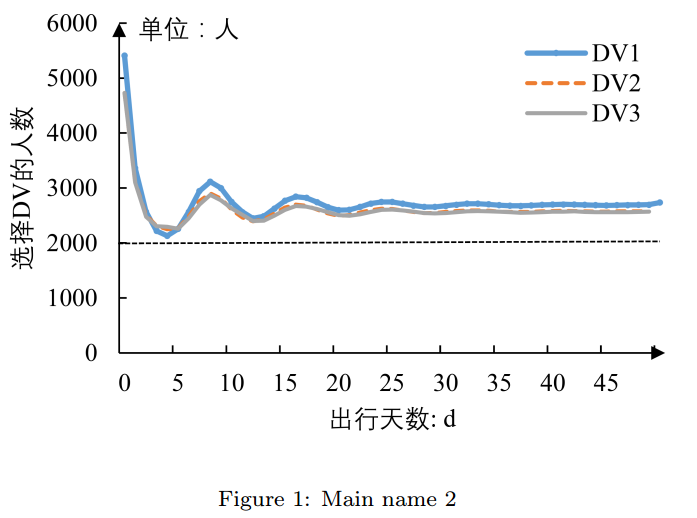
\includegraphics[width=0.7\textwidth]{./imgs/figure-1.png} %插入图片,[]中设置图片大小,{}中是图片文件名
	\caption{Main name 2} %最终文档中希望显示的图片标题
	\label{Fig.main1} %用于文内引用的标签
	\end{figure}

	\section{多图横排+默认编号}
	\begin{figure}[H]
	\centering  %图片全局居中
	\subfigure[name1]{
	\label{Fig.sub.1}
	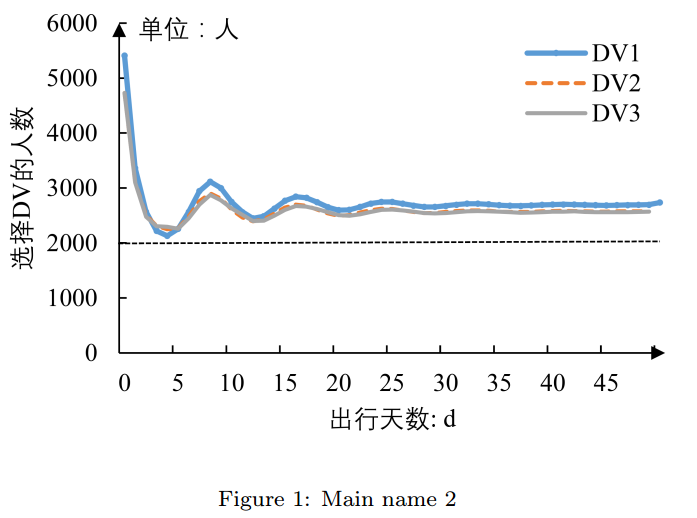
\includegraphics[width=0.45\textwidth]{./imgs/figure-1.png}}
	\subfigure[name2]{
	\label{Fig.sub.2}
	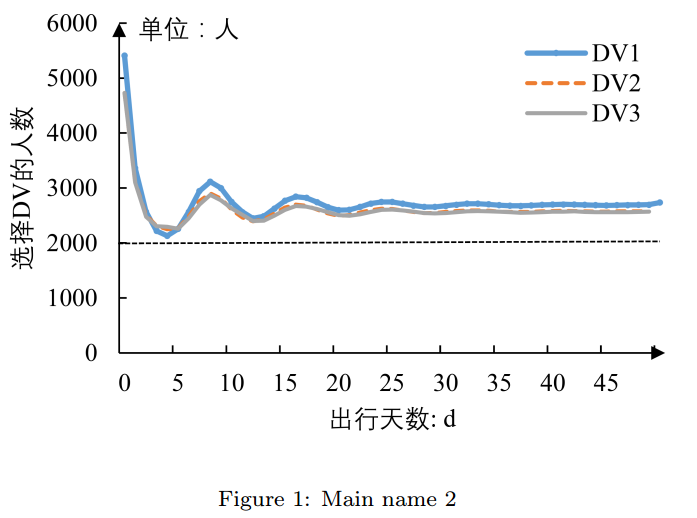
\includegraphics[width=0.45\textwidth]{./imgs/figure-1.png}}
	\caption{Main name}
	\label{Fig.main2}
	\end{figure}

	\section{多图横排+自定义编号}
	%注意:此段中在引用中增加了主图编号的引用
	Figure \ref{Fig.main3} has two sub-figures, fig. \ref{Fig.main3}\ref{Fig3.sub.1} is the travel demand of driving auto, and fig. \ref{Fig.main3}\ref{Fig3.sub.2} is the travel demand of park-and-ride.
	%以下code与上一小节的无变化
	\begin{figure}[H]
	\centering  %图片全局居中
	\subfigure[name1]{
	\label{Fig3.sub.1}
	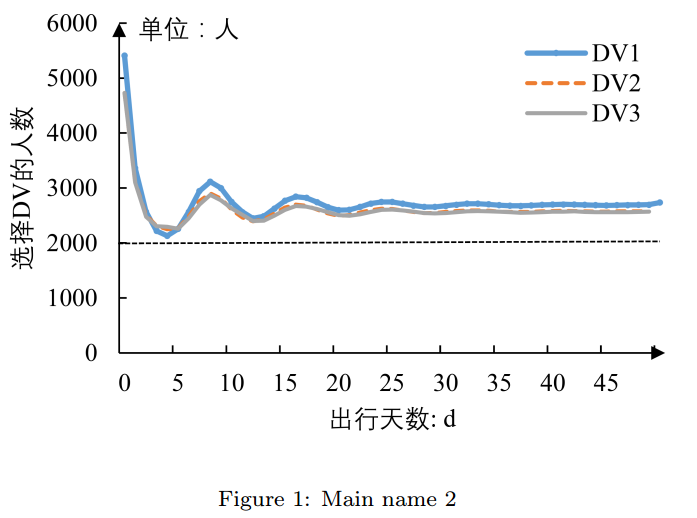
\includegraphics[width=0.45\textwidth]{./imgs/figure-1.png}}
	\subfigure[name2]{
	\label{Fig3.sub.2}
	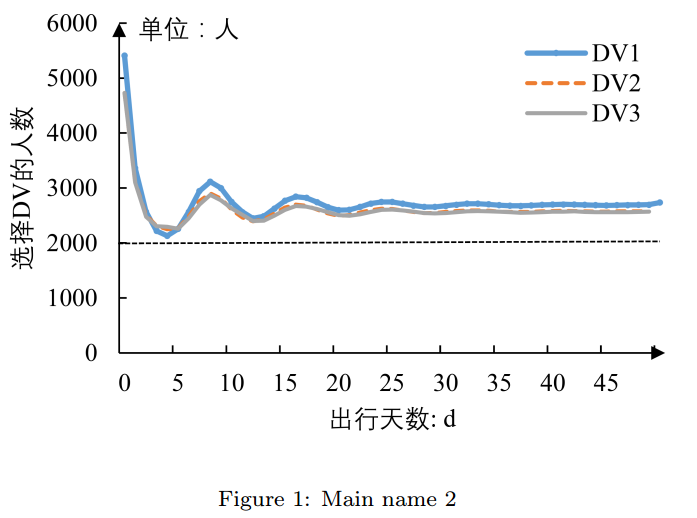
\includegraphics[width=0.45\textwidth]{./imgs/figure-1.png}}
	\caption{Main name}
	\label{Fig.main3}
	\end{figure}

	\section{多图并排显示(非子图模式)}
	\begin{figure}[H]
	\centering %图片全局居中
	%并排几个图,就要写几个minipage
	\begin{minipage}[b]{0.45\textwidth} %所有minipage宽度之和要小于1,否则会自动变成竖排
	\centering %图片局部居中
	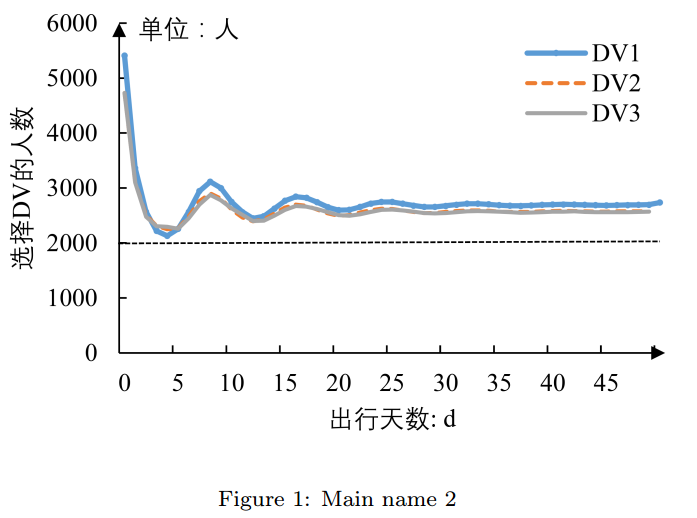
\includegraphics[width=0.8\textwidth]{./imgs/figure-1.png} %此时的图片宽度比例是相对于这个minipage的,不是全局
	\caption{name 1}
	\label{Fig.1}
	\end{minipage}
	\begin{minipage}[b]{0.45\textwidth} %所有minipage宽度之和要小于1,否则会自动变成竖排
	\centering %图片局部居中
	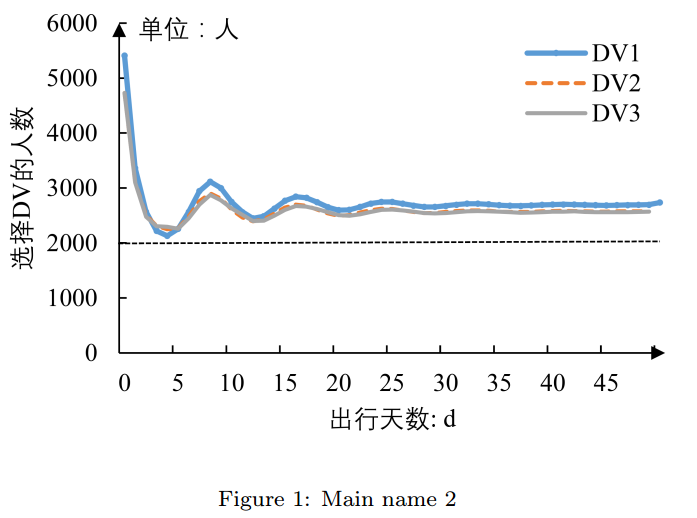
\includegraphics[width=0.8\textwidth]{./imgs/figure-1.png}%此时的图片宽度比例是相对于这个minipage的,不是全局
	\caption{name 2}
	\label{Fig.2}
	\end{minipage}
	\end{figure}

	\section{参考资料}
	\begin{itemize}
		\item \href{https://zhuanlan.zhihu.com/p/32925549}{LaTeX排版札记:part 4—插入图片(并排显示、自定义编号)}
	\end{itemize}
	
	% % % % % % % % % %
	\backmatter
	% 使用 bibLaTeX 制作书目
	\printbibliography[heading=bibintoc]
	
	% 图, 表索引. 可有可无.
	\listoffigures
	\listoftables

	% 制作索引 (用 imakeidx 的功能可以制作多份)
	{\footnotesize
	\indexprologue{中文术语按汉语拼音排序.}
	\printindex}
\end{document}
